% !TeX TXS-program:compile = txs:///pdflatex/[--shell-escape]

\pdfoptionpdfminorversion=5
\documentclass[27pt, aspectratio=169, t ,hyperref={pdfpagelabels=false}]{beamer}
\usepackage{pgfpages}
%\setbeameroption{show notes on second screen=right}



\mode<presentation> {
    \usetheme{HHUD}
    \setbeamercovered{invisible}
}
\usepackage[ngerman]{babel}
\usepackage[utf8]{inputenc}
\usepackage{times}
\usepackage[T1]{fontenc}
\usepackage{amsmath}
\usepackage{subfigure}
\usepackage{graphicx}
\usepackage{hyperref}
\usepackage{xmpmulti}
\usepackage{multicol}
\usepackage{icomma}
\usepackage{csquotes}
\usepackage{listings}
%\usepackage{minted} % Funktioniert grade noch nicht 
\usepackage[backend=biber,style=numeric,url=false]{biblatex}

\bibliography{references.bib}
% If you want to exclude the appendix from the frame counter you have to use the appendixnumberbeamer package. But be aware that the current version causes a problem with the frame counter.
\usepackage{appendixnumberbeamer}

%% Die folgenden Zeilen können auskommentiert werden, um vor jedem Kapitel eine Gliederungsfolie einzufügen
% \AtBeginSection[] {
%   \begin{frame}<beamer>
%     \thispagestyle{empty}
%     \frametitle{Gliederung}
%     \vspace{-5mm}
%     \tableofcontents[currentsection]
%   \end{frame}
% }

\usebackgroundtemplate{
\includegraphics[width=\paperwidth]{fig/Vorlagen/background_cd_2020}}

\newcommand{\backgroundNormal}{\usebackgroundtemplate{
    
\includegraphics[width=\paperwidth]{fig/Vorlagen/background_cd_2020}}}
\newcommand{\backgroundTitle}{\usebackgroundtemplate{
    
\includegraphics[width=\paperwidth]{fig/Vorlagen/background_heine}}}
\newcommand{\backgroundEmpty}{\usebackgroundtemplate{
    
\includegraphics[width=\paperwidth]{fig/Vorlagen/background_empty}}}
    
\setlength{\leftmargini}{9pt}
\setbeamersize{text margin left=25pt,text margin right=25pt} 
\setbeamertemplate{itemize/enumerate subbody end}{\vspace{.5\baselineskip}}

% =============== Meta-Daten =============== %
\title{Betriessystementwicklung:\\Shell-Implementierung und plattformunabhängige Apps}
\author{Carsten Krollmann}
\date{9.7.2025}
\institute{Institut für Informatik\\Heinrich-Heine-Universität Düsseldorf}
\subject{Informatik}

%
% Hier beginnt das Dokument
%


% =============== Eigene Präambel-Befehle =============== %
% Kopieren von Folien, wenn nur Bilder sich ändern
\usepackage{clipboard}


% Darstellung von Pseudocode
\usepackage{algorithm}
\usepackage{algpseudocode} 

% Darstellung der Tabelle
\usepackage{booktabs}

% Footnotes auf Seite ganz nach unten schieben
\usepackage[bottom]{footmisc}

% anzeigen von Unicode
\usepackage{listings}
\lstset{
    basicstyle=\ttfamily\footnotesize,
    columns=fullflexible,
    breaklines=true,
    tabsize=4
}


% Graphendarstellung
\usepackage{tikz}
\usetikzlibrary{intersections, 
  arrows.meta, 
  positioning, 
  shapes.geometric, 
  decorations.pathmorphing,
  calc
}

\usepackage{enumitem}% bessere aufzählungen
% Standartaufzählung wieder verwenden
\setlist[itemize,1]{label=\textbullet}
\setlist[itemize,2]{label=--}
\setlist[itemize,3]{label=$\ast$}


% Schriftgröße der Zitierungen
% fontsize{x}{y} gibt x pt Schriftgröße und y pt Zeilenabstand
\renewcommand{\footcite}[1]{%
  \footnote{%
    \fontsize{6}{8}\selectfont%
    \fullcite{#1}%
  }%
}

% Counter gegen Footnote duplicates
\newcounter{fnnumber} 


% Gedankenblasen-Makro
\newcommand{\gedankenblase}[6]{%
  \begin{scope}
    \small
    % Hauptblase
    \draw[fill=#4!60, draw=#5, thick] (#1,#2) ellipse (2cm and 1cm);
    \node at (#1,#2) {\parbox{3cm}{\centering #3}};
    % Punkte nach unten
    \draw[fill=#4!50, draw=#5] (#1+1*#6,#2-1.15) circle (0.2cm);
    \draw[fill=#4!30, draw=#5] (#1+1.3*#6,#2-1.5) circle (0.1cm);
  \end{scope}
}


% ===============    =============== %



\begin{document}

\backgroundTitle
  \begin{frame}
    \thispagestyle{empty}
    \begin{columns}
    \column{0.4\paperwidth}
    {
    \footnotesize
    \color{hhuBlau}
    \put(20,-200){\insertdate}
    
    }
    \column{0.6\paperwidth}
    
    \color{hhuBlau}
    \LARGE \inserttitle\\[\baselineskip]
    
    \large \insertauthor
    \end{columns}
  \end{frame}
  \backgroundNormal


  \begin{frame}
    \thispagestyle{empty}
    \frametitle{Gliederung}
    \vspace{-5mm}
    \tableofcontents
  \end{frame}

  % % % % % % % % % % Ab hier werden die LaTeX-Dateien der einzelnen Abschnitte eingefügt % % % % % % % % % %

  \section{Einleitung - Ziele und Motivation}


\begin{frame}{Motivation}
    \begin{Large}
        Apps sind auf Betriebssystem angewiesen \newline
        $\Rightarrow$ starke Abhängigkeit \newline
        \newline
        \onslide<2,3>
        Apps auf unterschiedlichen Systemen \newline
        $\Rightarrow$ enge Schnittstelle \newline
        \onslide<3>
        \newline
        \textcolor{gray}{Beispiel: Syscalls $\Rightarrow$ ein einziger Interrupt}
    \end{Large}
\end{frame}


\begin{frame}{Ziele}
    \begin{Large}
        Ziele:
    \end{Large}
    \vspace{15pt}

    \begin{itemize}
        \item Schnittstelle als Lib
        \item Kernel implementiert Schnittstelle
        \item Apps über Schnittstelle
        \item [] \quad $\Rightarrow$ Systeme austauschbar
    \end{itemize}
\end{frame}


\begin{frame}{Struktur}
    \begin{center}
        \begin{tikzpicture}[node distance=1.2cm and 1cm, every node/.style={minimum width=2.2cm, minimum height=0.9cm, align=center, font=\small}]

        % Farben definieren
        \tikzstyle{app}=[draw, fill=blue!20, ellipse]
        \tikzstyle{lib}=[draw, fill=orange!30, diamond, rounded corners]
        \tikzstyle{kernel}=[draw, fill=green!25, rectangle, aspect=2]

        % Apps
        \node[app] (app1) {App A};
        \node[app, right=of app1] (app2) {App B};
        \node[draw=none, right=of app2] (dots) {\Large$\cdots$};
        \node[app, right=of dots] (app3) {App N};

        % Userlib
        % Userlib – zentriert zwischen app1 und app3
        \node[lib, below=1cm of $(app1)!0.5!(app3)$] (userlib) {Userlib\\(Usermode)};

        % Kernel
        \node[kernel, below left=0.8cm and 1.2cm of userlib] (kernel1) {Kernel 1};
        \node[kernel, below right=0.8cm and 1.2cm of userlib] (kernel2) {Kernel 2};

        % Geschwungene Verbindungen Apps -> Userlib (ungerichtet)
        \draw[->] (app1.south) to[out=-90, in=135] node[midway, above, yshift=-5pt] {API} (userlib.north west);
        \draw[->] (app2.south) to[out=-90, in=90] node[near end, above, yshift=-5pt] {API} (userlib.north);
        \draw[->] (app3.south) to[out=-90, in=45] node[midway, above, yshift=-5pt] {API} (userlib.north east);


        % Userlib → Kernel
        \draw[->] (userlib.south west) to[out=-100, in=90] node[near end, above, yshift=-5pt] {Syscalls} (kernel1.north);
        \draw[->] (userlib.south east) to[out=-80, in=90] node[near end, above, yshift=-5pt] {Syscalls} (kernel2.north);
        \end{tikzpicture}
    \end{center}
\end{frame}


  \section{Userlib Schnittstelle}



\begin{frame}{Userlib}
    \begin{Large}
        Userlib als Grundlage für Schnittstelle
    \end{Large}
    \vspace{15pt}

    \begin{itemize}
        \item Kapselung des Kernels
        \item Apps nur gegen Userlib
        \item Verbindung zu Kernel via Syscalls
    \end{itemize}
    
\end{frame}


\begin{frame}{Userlib}
    \begin{Large}
        $\Rightarrow$ Beide Kernel implementieren Userlib \newline \newline
        $\Rightarrow$ Apps laufen unabhänging
    \end{Large}
    \vspace{15pt}
\end{frame}


\begin{frame}{Userlib Erweiterung}
    \begin{Large}
        Erweiterung der lib: {\tiny \cite{usrlib-repo}}
    \end{Large}
    \vspace{15pt}

    \begin{itemize}
        \item mehr Syscalls
        \item Wrapper um die Syscalls
        \item Runtime \& Environment
        \item Musik
        \item Bilder
        \item System Management
    \end{itemize}
\end{frame}


\begin{frame}{Userlib Aufbau}
    \begin{Large}
        Aufbau: \tiny \cite{usrlib-repo}
    \end{Large}
    \vspace{5pt}
    

    \begin{minipage}[t]{0.48\textwidth}
        \centering
        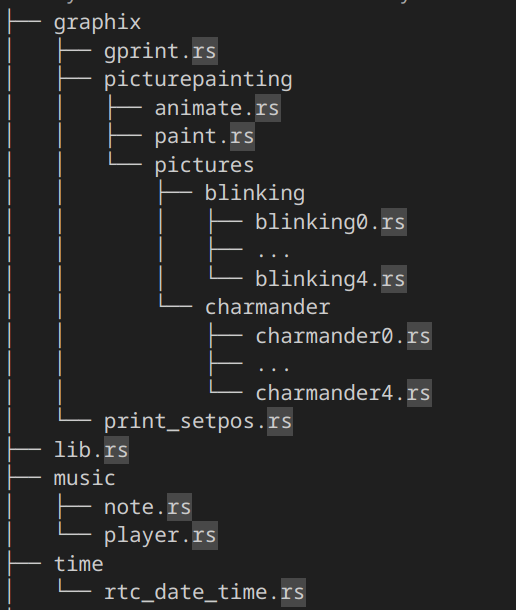
\includegraphics[height=0.7\textheight]{fig/Code Screens/Tree 1.png} 
    \end{minipage}
    \hfill
    \begin{minipage}[t]{0.48\textwidth}
        \centering
        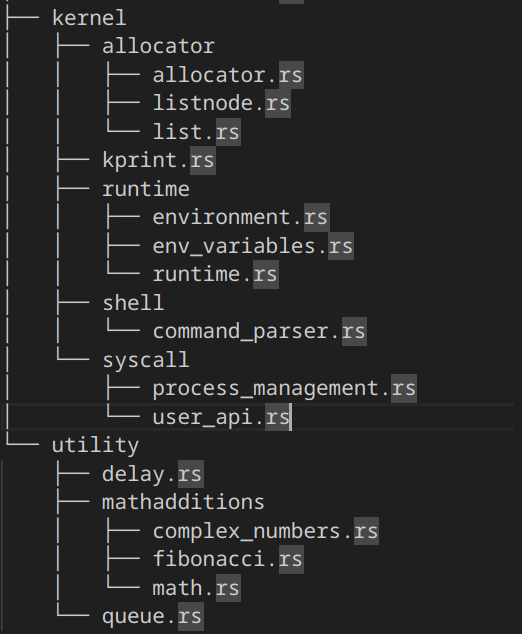
\includegraphics[height=0.7\textheight]{fig/Code Screens/Tree 2.png} 
    \end{minipage}
\end{frame}



\begin{frame}{Userlib Aufbau}
    \begin{minipage}[t]{0.3\textwidth}
        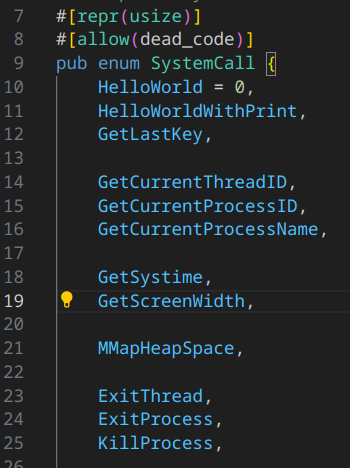
\includegraphics[height=0.8\textheight]{fig/Code Screens/Enum1.png} 
    \end{minipage}
    \hfill
    \begin{minipage}[t]{0.65\textwidth}
        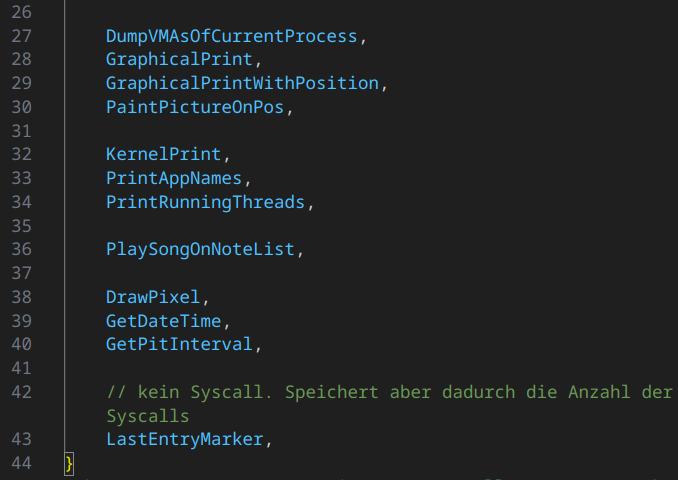
\includegraphics[height=0.8\textheight]{fig/Code Screens/Enum2.png} 
    \end{minipage}
\end{frame}

  \section{Shellfunktion}


\begin{frame}{Shell}
    \begin{Large}
        Shell läuft im Kernel
    \end{Large}
    \vspace{15pt}

    \begin{itemize}
        \item Liest Tastatur aus
        \item setzt Befehle zusammen
    \end{itemize}
    
\end{frame}


\begin{frame}{Shell}
    \begin{Large}
        Shellfunktion: 
    \end{Large}
    \vspace{15pt} 
    
    \begin{itemize}
        \item Erfassen der Eingabe
        \item parsen der Befehle
        \item [] \begin{itemize}
            \item Argumente zerpflücken
            \item Environment-Variabeln Management
        \end{itemize}
        \item starten der Apps
        \item [] \begin{itemize}
            \item App wird geladen
            \item Scheduler richtet Prozess ein
            \item Neuer Thread (Mapping + Environment)
        \end{itemize}
    \end{itemize}
\end{frame}



  \section{Apps}



\begin{frame}{Apps Liste}
    \begin{Large}
        Folgende Apps wurden implementiert
    \end{Large}
    \vspace{15pt}

    \begin{itemize}
        \item animation
        \item apps
        \item datetime
        \item echo
        \item kill
        \item mandelbrot
        \item music
        \item pic
        \item threads
        \item uptime
    \end{itemize}
    
\end{frame}



  \section{Demo}

\begin{frame}{Demo Apps}
    \begin{Large}
        Folgende Apps werden vorgeführt
    \end{Large}
    \vspace{15pt}

    \begin{itemize}
        \item animation (visuell)
        \item music (audio)
        \item threads (management)
        \item kill (management)
    \end{itemize}
    
\end{frame}


\begin{frame}{Demo App}
    \begin{Large}
        Laufen Apps jetzt auch unabhängig?
    \end{Large}
    \vspace{15pt} 
    
    $\Rightarrow$ Zeige an music app
\end{frame}




  
  %\printbibliography

  
  \appendix
  % anhang mit Quellenverzeichniss
  \section{Anhang}

\begin{frame}[allowframebreaks]{Quellenangaben}
    \printbibliography
\end{frame}




  

  % % % % % % % % % % Ende der eingefügten LaTeX-Dateien % % % % % % % % % %

\end{document}

%
% Hier endet das Dokument
%
